\section{Behaviors}
\label{sec:Behaviors}

The three behaviors described in Section~\ref{sec:Introduction} are described and presented in pseudocode in this section. These algorithms were designed for a system which meet the following assumptions:
\begin{itemize}
	\item 3D cubic lattice movement according to either Pivoting Cube Model or Sliding Cube Model.
	\item Each module can detect a unique ID number and a relative orientation for each connector face.
	\item Modules are able to send simple messages through their connecting faces to other modules.
\end{itemize}

%%%%%%%%%%%%%%%%%%%%%%%%%%%%%%%%%%%%%%%%%%%%%%%%%%%%%%%%%%%%%%%%%%%%%%%%%%%%%%%%%%%%%%%%%%%%%%%%%%%%%%%%%%%%%%%%%%%%%%%%%%%%%%%%%%%%%%%%%%%%%%%
%%%%%%%%%%%%%%%%%%%%%%%%%%%%%%%%%%%%%%%%%%%%%%%%%%%%%%%%%%%%%%%%%%%%%%%%%%%%%%%%%%%%%%%%%%%%%%%%%%%%%%%%%%%%%%%%%%%%%%%%%%%%%%%%%%%%%%%%%%%%%%%
\subsection{Path Following Behavior}
\label{sec:algArrow}
%%%%%%%%%%%%%%%%%%%%%%%%%%%%%%%%%%%%%%%%%%%%%%%%%%%%%%%%%%%%%%%%%%%%%%%%%%%%%%%%%%%%%%%%%%%%%%%%%%%%%%%%%%%%%%%%%%%%%%%%%%%%%%%%%%%%%%%%%%%%%%%
%%%%%%%%%%%%%%%%%%%%%%%%%%%%%%%%%%%%%%%%%%%%%%%%%%%%%%%%%%%%%%%%%%%%%%%%%%%%%%%%%%%%%%%%%%%%%%%%%%%%%%%%%%%%%%%%%%%%%%%%%%%%%%%%%%%%%%%%%%%%%%%

The goal of this behavior is guide mobile modules to follow paths described by fiducials embedded in in adjacent modules' lattice connection points. This behavior requires that  each module can determine from each of its neighbor connection interfaces a desired direction relative to its current absolute location that the module should move towards. The simplest implementation of this path following behavior involves passive hard-coded "arrow tags" in a lattice of passive modules, similar to arrows embedded along a road, as in Figure~\ref{fig:intro}a-b. Path following behavior is then extended to modules which have connection face identities which are globally uniquely defined, and which contain some embedded "direction" or ability to determine the relative connection angle. Modules can then receive a mapping of ID numbers and "directions", and then can follow a virtually created path along a configuration of modules. A path could be defined along the surface of a large partially assembled aggregate of modules to guide modules to desired attachment points, similar to how optimization technique following gradient descent paths to reach a goal.

%%%%%%%%%%%%%%%%%%%%%%%%%%%%%%%%%%%%%%%%%%%%%%%%%%%%%%%%%%%%%%%%%%%%%%%%%%%%%%%%%%%%%%%%%%%%%%%%%%%%%%%%%%%%%%%%%%%%%%%%%%%%%%%%%%%%%%%%%%%%%%%	
\setcounter{algorithm}{-1}
\begin{algorithm}
	 
	\caption{Path Following Algorithm}
	\label{algorithmArrow}
	
	\SetAlgoLined
%	\KwData{M-Blocks 3D}
	initialization\;
	\While{Connected to valid module}
	{
		determine arrow direction\;
		\eIf{Flywheel plane is aligned with arrow}
		{
			Move in direction of arrow\;
		}
		{
			Attempt to align flywheel with correct plane\;
		}
	}
	\caption{This algorithm attempts to drive a cube in the direction of the embedded direction defined by the \tagNamePlural.}
\end{algorithm}
%%%%%%%%%%%%%%%%%%%%%%%%%%%%%%%%%%%%%%%%%%%%%%%%%%%%%%%%%%%%%%%%%%%%%%%%%%%%%%%%%%%%%%%%%%%%%%%%%%%%%%%%%%%%%%%%%%%%%%%%%%%%%%%%%%%%%%%%%%%%%%%

%%%%%%%%%%%%%%%%%%%%%%%%%%%%%%%%%%%%%%%%%%%%%%%%%%%%%%%%%%%%%%%%%%%%%%%%%%%%%%%%%%
%%%%%%%%%%%%%%%%%%%%%%%%%%%%%%%%%%%%%%%%%%%%%%%%%%%%%%%%%%%%%%%%%%%%%%%%%%%%%%%%%%%%%%%%%%%%%%%%%%%%%%%%%%%%%%%%%%%%%%%%%%%%%%%%%%%%%%%%%%%%%%%
\subsection{3D Line Formation Behavior}
\label{ssec:algline}
%%%%%%%%%%%%%%%%%%%%%%%%%%%%%%%%%%%%%%%%%%%%%%%%%%%%%%%%%%%%%%%%%%%%%%%%%%%%%%%%%%%%%%%%%%%%%%%%%%%%%%%%%%%%%%%%%%%%%%%%%%%%%%%%%%%%%%%%%%%%%%%
%%%%%%%%%%%%%%%%%%%%%%%%%%%%%%%%%%%%%%%%%%%%%%%%%%%%%%%%%%%%%%%%%%%%%%%%%%%%%%%%%%%%%%%%%%%%%%%%%%%%%%%%%%%%%%%%%%%%%%%%%%%%%%%%%%%%%%%%%%%%%%%


The goal of this algorithm is to reconfigure an arbitrary 3D configuration of modules into a line using a decentralized algorithm. Initially a centralized or specially selected module selects to be the "seed" module for the line.  In contrast to centralized line formation algorithms as in~\cite{sung2015reconfiguration}, this work implements the algorithm described in Algorithm~\ref{algorithmLine}. This behavior can be implemented in several ways, but in this work each modules uses knowledge of its direct neighbors, and very simple communication between the faces of adjacent modules. These communications are implemented as as a binary "connect here" or "keep moving," using visible light sensors and LED's on the modules' faces. Future versions could  incorporate the path following behavior to optimize the movement efficiency (i.e. assembly speed) for a group of modules.

%%%%%%%%%%%%%%%%%%%%%%%%%%%%%%%%%%%%%%%%%%%%%%%%%%%%%%%%%%%%%%%%%%%%%%%%%%%%%%%%%%%%%%%%%%%%%%%%%%%%%%%%%%%%%%%%%%%%%%%%%%%%%%%%%%%%%%%%%%%%%%%
\setcounter{algorithm}{0}
\begin{algorithm}[ht] 
	%\hrulefill
	\caption{Line formation Algorithm}
	\label{algorithmLine}
	\SetAlgoLined
	Initialization\;
	\While{line seed not selected by Server}
	{
		Modules send wireless information about their neighbors\;
		server searches for longest existing line\;
	}
	\While{Not part of line}
	{
		Update sensors and state\;
		\eIf{Neighbors = 1 and movement possible}
		{
			Move in a consistent direction \;
		}
		{
			Attempt to align flywheel with correct plane\;
		}
	}
	\caption{This algorithm attempts to turn a 3D shape configuration of modules into a line. The algorithm runs in a decentralized manner except for the initial step which uses a centralized "Server" block which communicated through WiFi which module is the "seed" of the line. }
\end{algorithm}
%%%%%%%%%%%%%%%%%%%%%%%%%%%%%%%%%%%%%%%%%%%%%%%%%%%%%%%%%%%%%%%%%%%%%%%%%%%%%%%%%%%%%%%%%%%%%%%%%%%%%%%%%%%%%%%%%%%%%%%%%%%%%%%%%%%%%%%%%%%%%%%




%%%%%%%%%%%%%%%%%%%%%%%%%%%%%%%%%%%%%%%%%%%%%%%%%%%%%%%%%%%%%%%%%%%%%%%%%%%%%%%%%%%%%%%%%%%%%%%%%%%%%%%%%%%%%%%%%%%%%%%%%%%%%%%%%%%%%%%%%%%%%%%
%%%%%%%%%%%%%%%%%%%%%%%%%%%%%%%%%%%%%%%%%%%%%%%%%%%%%%%%%%%%%%%%%%%%%%%%%%%%%%%%%%%%%%%%%%%%%%%%%%%%%%%%%%%%%%%%%%%%%%%%%%%%%%%%%%%%%%%%%%%%%%%
\subsection{Light Gradient Aggregation Behavior}
\label{sec:algLight}
%%%%%%%%%%%%%%%%%%%%%%%%%%%%%%%%%%%%%%%%%%%%%%%%%%%%%%%%%%%%%%%%%%%%%%%%%%%%%%%%%%%%%%%%%%%%%%%%%%%%%%%%%%%%%%%%%%%%%%%%%%%%%%%%%%%%%%%%%%%%%%%
%%%%%%%%%%%%%%%%%%%%%%%%%%%%%%%%%%%%%%%%%%%%%%%%%%%%%%%%%%%%%%%%%%%%%%%%%%%%%%%%%%%%%%%%%%%%%%%%%%%%%%%%%%%%%%%%%%%%%%%%%%%%%%%%%%%%%%%%%%%%%%%
This goal of this behavior is to implement essentially a Braitenberg phototaxis behavior for lattice based modular robots, i.e. aggregating robots towards a light source. The algorithm assumes modules begin not connected to a lattice and continue to move towards light until they reach a specific "goal" structure defined by a specific aggregate of modules, which ensures that there is only a single successful aggregate. The modules move until they connect to a module that indicates it is part of the goal unit through some simple form of neighbor to neighbor communication, i.e. the face is lighted. With the exception of some method for selecting a single seed module, this algorithm is entirely distributed, and only depends on local information. This algorithm is based on the work from Claici et. al in~\cite{claici2017distributed}, but is refined in this work to account for some of the nuances of the actual hardware system.


%%%%%%%%%%%%%%%%%%%%%%%%%%%%%%%%%%%%%%%%%%%%%%%%%%%%%%%%%%%%%%%%%%%%%%%%%%%%%%%%%%%%%%%%%%%%%%%%%%%%%%%%%%%%%%%%%%%%%%%%%%%%%%%%%%%%%%%%%%%%%%%
\setcounter{algorithm}{1}
\begin{algorithm}[htbp] 
	%\hrulefill
	\caption{Light guided aggregation Algorithm}
	\label{algorithmAggregate}
	\SetAlgoLined
	%	\Kw{M-Blocks 3D}
	%	initialization\;
	\While{Not connected to Goal Configuration}
	{
		Update State read sensors\;
		\uIf{Numer of Neighbors  = 0}
		{
			Roll in direction of the brightest face that isn't on top\;
		}
		\uElseIf{Neighbors = 1, but not at Goal}
		{
			Run algorithm to attempt to move towards light as a group\;
		}
		\uElseIf{Neighbors = 2, but not at Goal}
		{
			Disconnect from structure
		}
	}
	\caption{This algorithm attempts to drive a group of modules to form a single aggregated group based guided by a light gradient.}
\end{algorithm}
%%%%%%%%%%%%%%%%%%%%%%%%%%%%%%%%%%%%%%%%%%%%%%%%%%%%%%%%%%%%%%%%%%%%%%%%%%%%%%%%%%%%%%%%%%%%%%%%%%%%%%%%%%%%%%%%%%%%%%%%%%%%%%%%%%%%%%%%%%%%%%%


The experiments are implemented by placing a light source in a corner of a rectangular arena, and providing a \emph{seed} module  to designate the correct location to connect to. One possible biological inspiration for this experiment is to imagine that the modules are cells of a plant, and the algorithm is to grow a structure towards the light source as a plant. As far as we know this work would be the first to accomplish this task in 3 dimensions using modular robots.
















%
%\begin{figure}[h]  
%	\centering
%	
%	\begin{subfigure}[b]{0.3\linewidth}
%		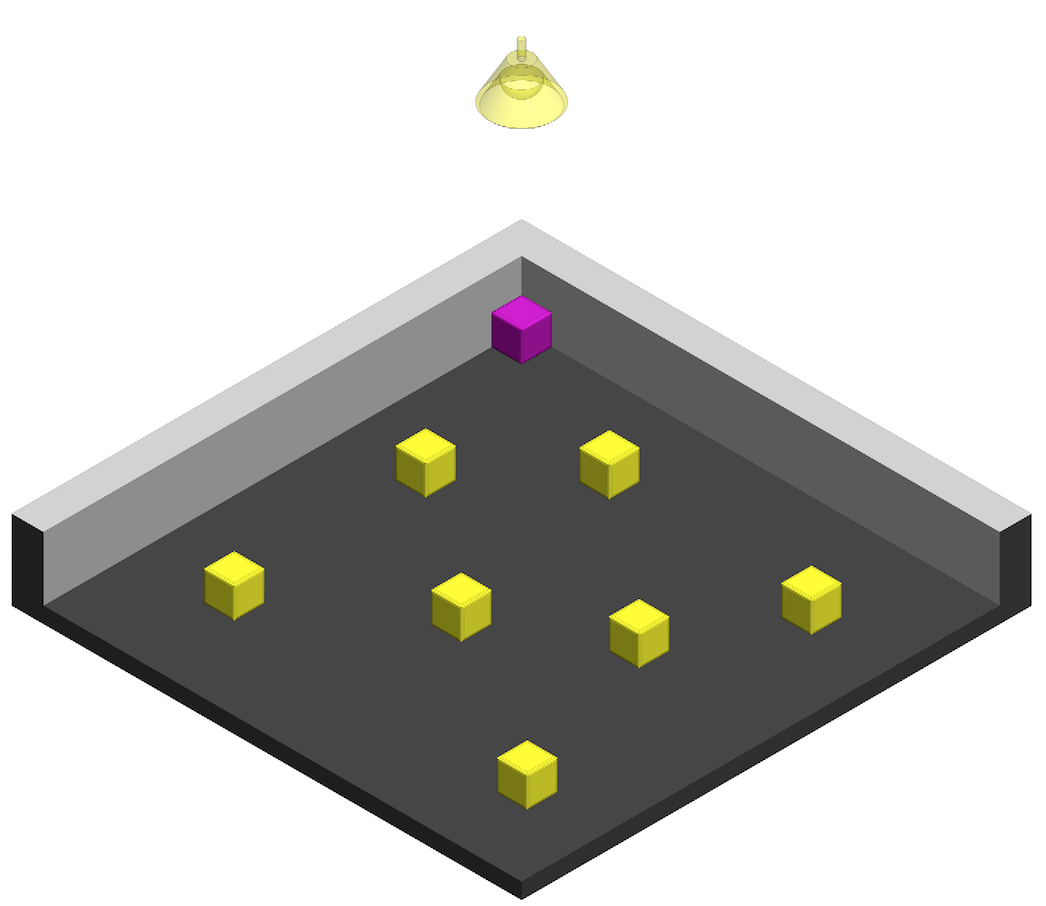
\includegraphics[width=0.9\linewidth]{figures/light_1.png}
%		\subcaption{} 
%	\end{subfigure}
%	\begin{subfigure}[b]{0.3\linewidth}
%		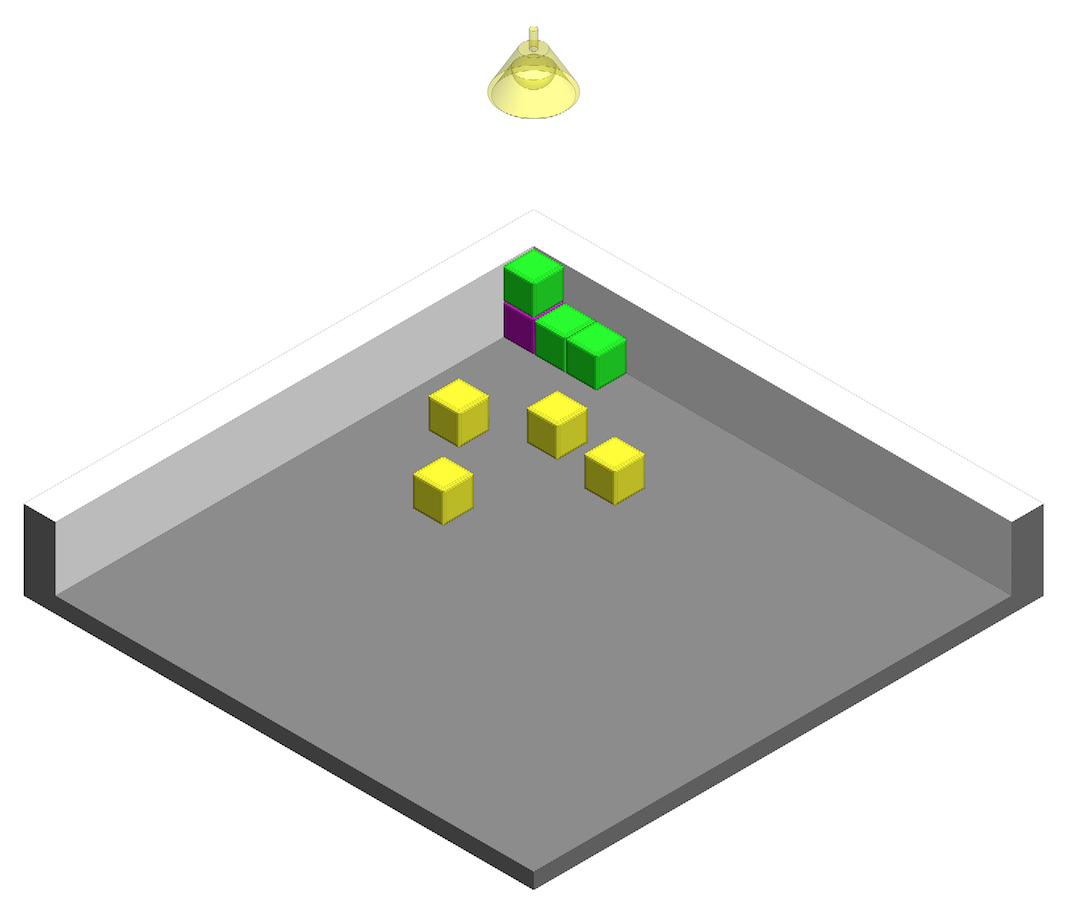
\includegraphics[width=0.9\linewidth]{figures/light_2.png}
%		\subcaption{} 
%	\end{subfigure}
%	\begin{subfigure}[b]{0.3\linewidth}
%		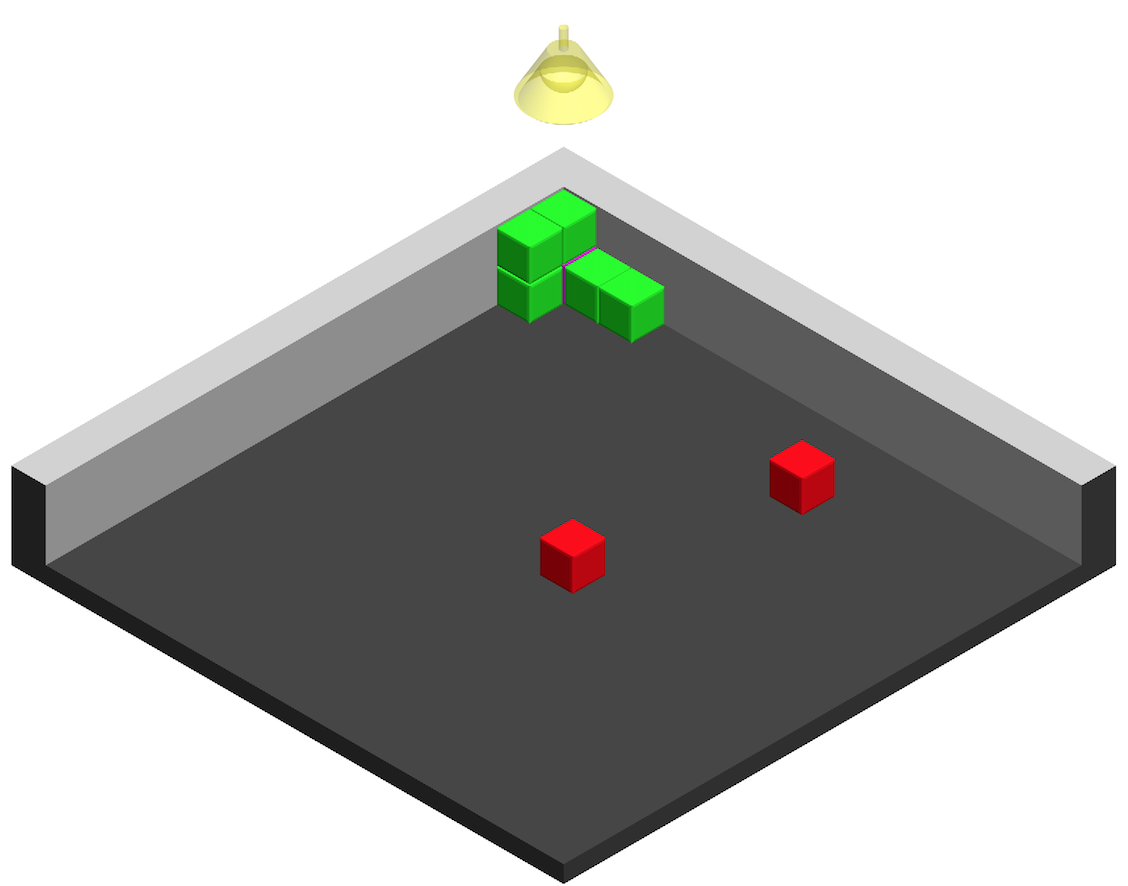
\includegraphics[width=0.9\linewidth]{figures/light_3.png}
%		\subcaption{} 
%	\end{subfigure}
%	
%	\caption{Three frames from an a illustration of the light-seeking experiment. One seed cube \emph{purple} is placed near the light, and the cubes in \emph{yellow} attempt to move towards the light. In the final frame, the modules which are in \emph{green} successfully reached the goal, while modules that are \emph{red} did not manage to join the target structure.}
%	
%	\label{fig:light}
%\end{figure}

%begin{figure}[h]  
%\centering
%
%\begin{subfigure}[b]{0.3\linewidth}
%	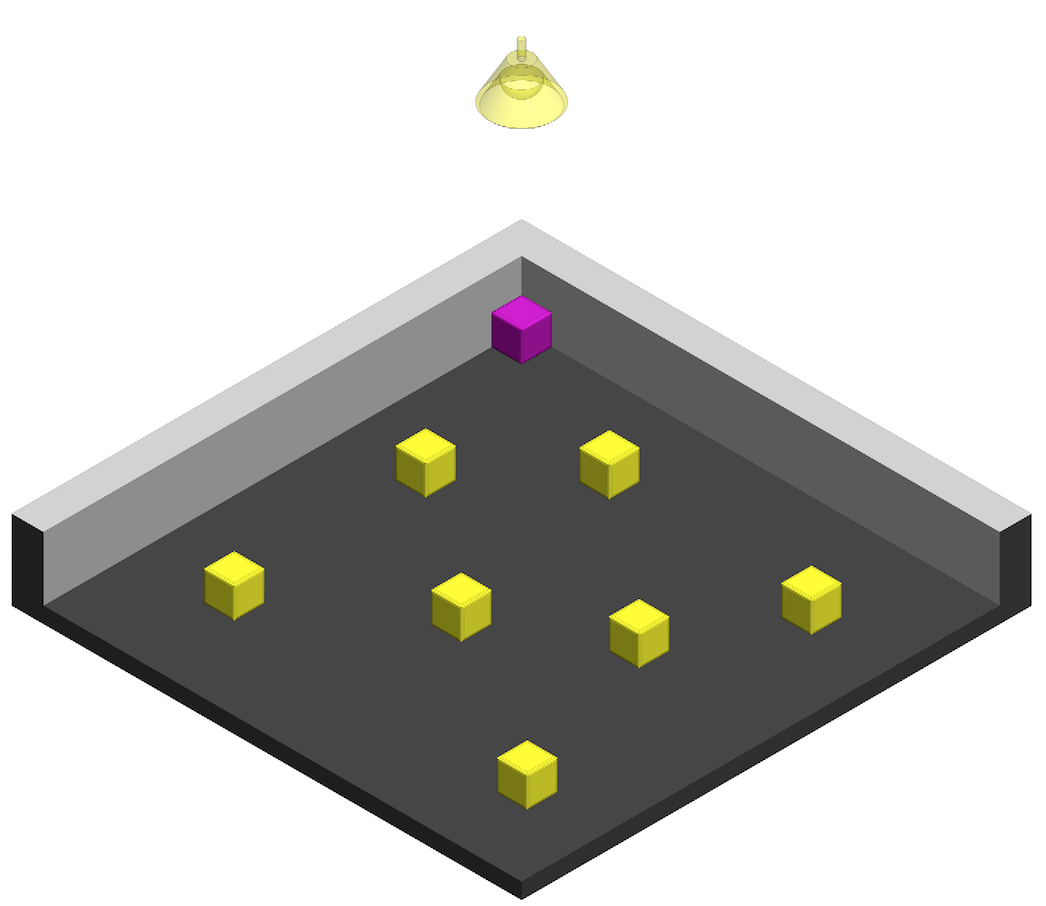
\includegraphics[width=0.9\linewidth]{figures/light_1.png}
%	\subcaption{} 
%\end{subfigure}
%\begin{subfigure}[b]{0.3\linewidth}
%	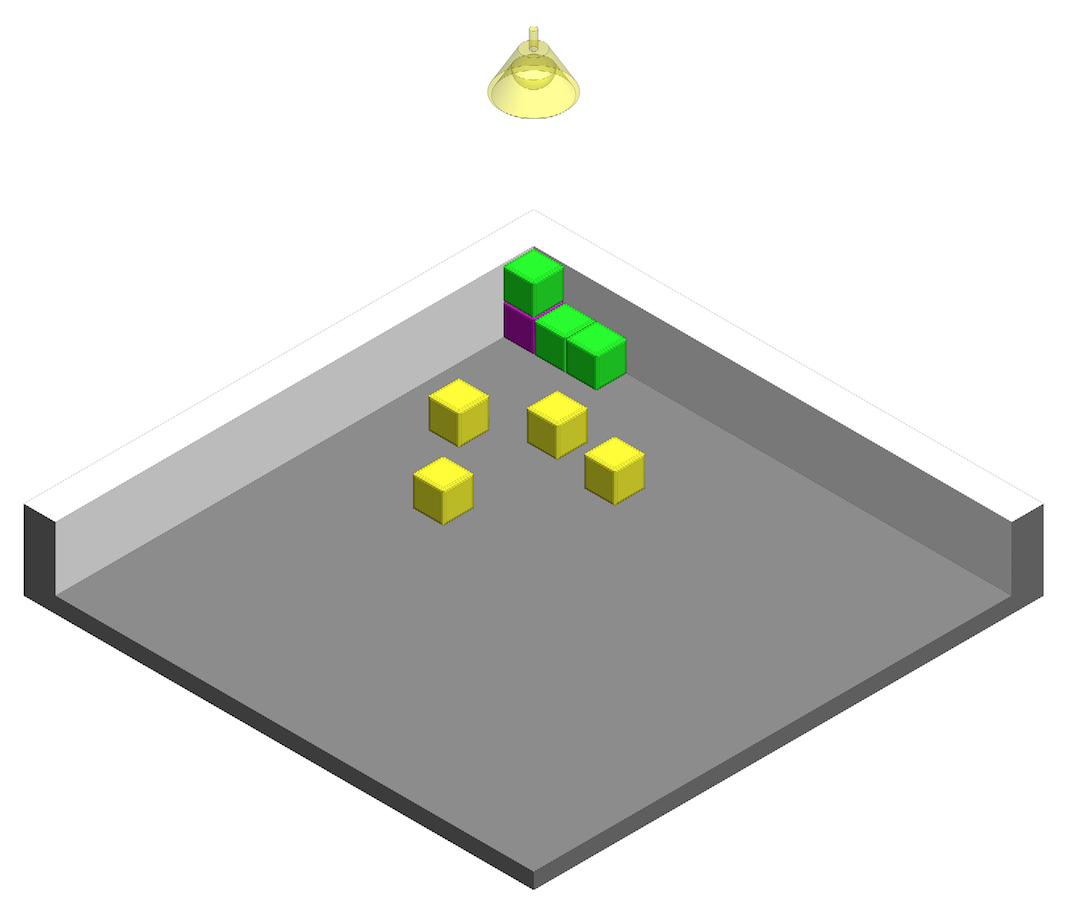
\includegraphics[width=0.9\linewidth]{figures/light_2.png}
%	\subcaption{} 
%\end{subfigure}
%\begin{subfigure}[b]{0.3\linewidth}
%	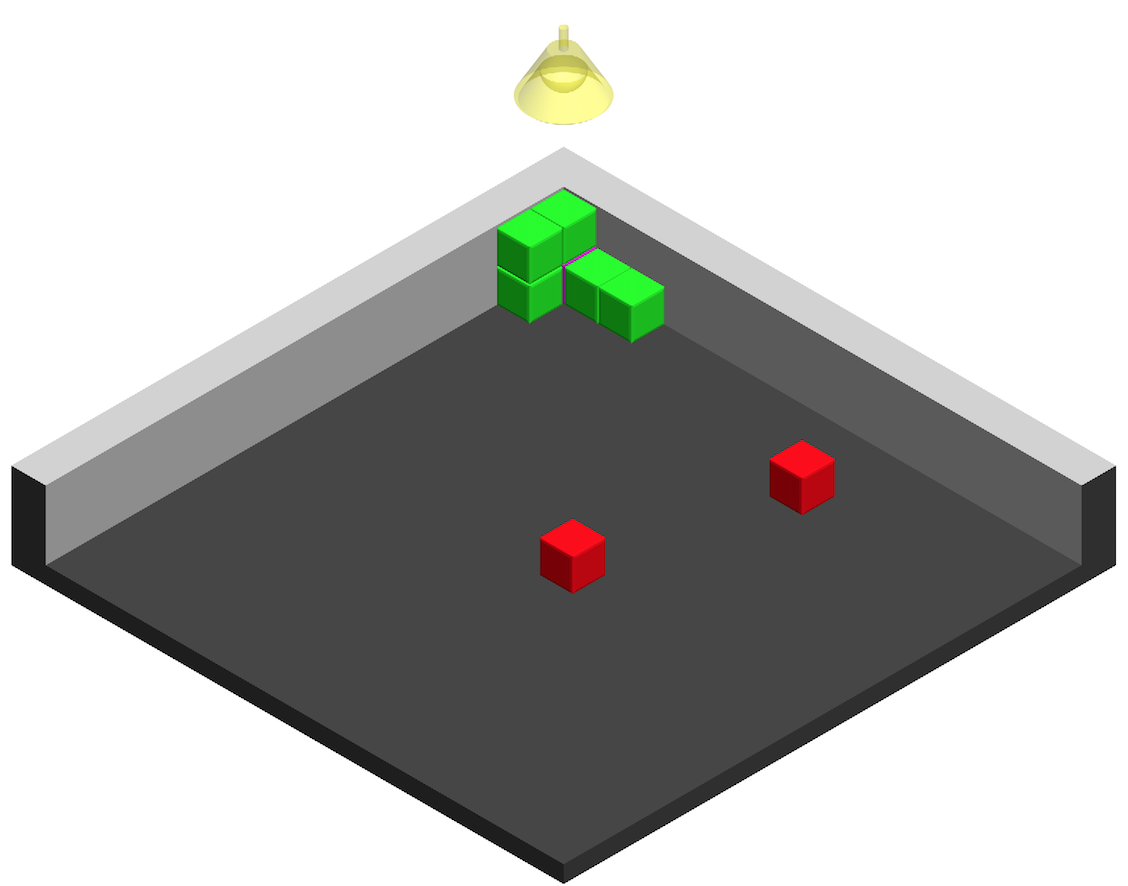
\includegraphics[width=0.9\linewidth]{figures/light_3.png}
%	\subcaption{} 
%\end{subfigure}
%
%\caption{Three frames from an a illustration of the light-seeking experiment. One seed cube \emph{purple} is placed near the light, and the cubes in \emph{yellow} attempt to move towards the light. In the final frame, the modules which are in \emph{green} successfully reached the goal, while modules that are \emph{red} did not manage to join the target structure.}
%
%\label{fig:light}
%\end{figure}

%
%\begin{figure}[h]  
%	\centering
%	\begin{subfigure}[b]{0.3\linewidth}
%		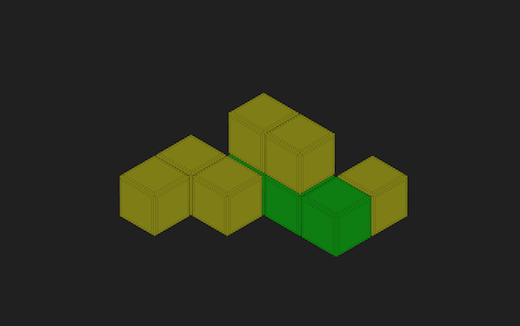
\includegraphics[width=0.9\linewidth]{figures/line_1.png}
%		\subcaption{} 
%	\end{subfigure}
%	\begin{subfigure}[b]{0.3\linewidth}
%		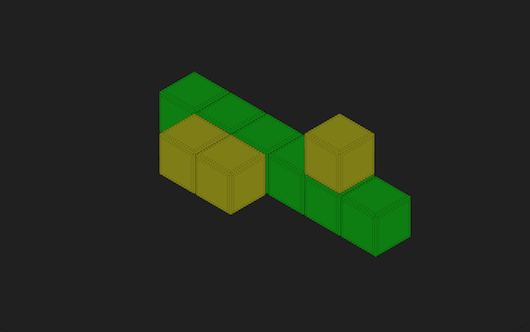
\includegraphics[width=0.9\linewidth]{figures/line_2.png}
%		\subcaption{} 
%	\end{subfigure}
%	\begin{subfigure}[b]{0.3\linewidth}
%		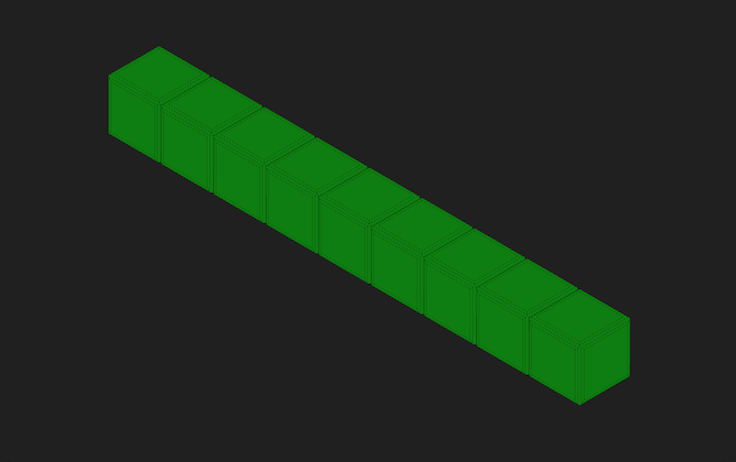
\includegraphics[width=0.9\linewidth]{figures/line_3.png}
%		\subcaption{} 
%	\end{subfigure}
%	
%	\caption{This experiment shows a random 3D configuration of M-Blocks reconfiguring into a line.}
%	
%	\label{fig:line}
%\end{figure}